\documentclass[a4paper,10pt,twoside]{article}

\usepackage[utf8]{inputenc}
\usepackage{enumitem}
\usepackage{moreenum}
\usepackage{graphicx}
\usepackage{fancyref}
\usepackage{multirow}
\usepackage{hyperref}
\usepackage[normalem]{ulem}
\usepackage[title]{appendix}
\usepackage{listings}

\textheight25.0cm
\textwidth16cm
\topmargin-.5cm
\oddsidemargin 0.cm
\evensidemargin 0.cm
\headheight0.5cm
\headsep0.cm
\footskip0.7cm
%\footheight2.5cm
\marginparwidth1.2cm
\marginparsep0.3cm

%%%%%%%%%%%%%%%%%%%%%%%%%%%%%%%%%%%%%%%%%%%%%%%%% END of HEADER

\title{DAVAÏ User Guide}
\author{A. Mary}
\date{\today}

\pdfinfo{%
  /Title    (Ugr)
  %/Author   (A. mary)
  /Creator  ()
  /Producer ()
  /Subject  ()
  /Keywords ()
}

\begin{document}
\maketitle

\tableofcontents
\vspace{1cm}
\newpage


DAVAÏ embeds the whole workflow from the source code to the green/red light validation status: fetching sources from Git, building executables, running test cases, analysing the results and displaying them on a dashboard.

For now, the only build system embedded is \texttt{gmkpack}, but we expect other systems to be plugged if required. In this version too, all main source projects are also supposed to be in the same repository. The next version of the DAVAÏ system will include multi-projects/repositories fetching, using the \textit{\texttt{bundle}} concept.

The dimensioning of tests (grid sizes, number of observations, parallelization...) is done in order to conceal representativity and execution speed. Therefore, in the general usecases, the tests are supposed to run on HPC. A dedicated usecase will target smaller configurations to run on workstation.\\

An accessible source code forge is to be set within the ACCORD consortium to host the central repository on which updates and releases are published, and where integration requests will be posted, reviewed and monitored. This is expected to be setup and advertised for 2022.
An update of the documentation with details about these aspects will be released in due time.



\newpage
\section{Systematic test of contributions}

\subsection{TUTORIAL: Test a contribution} 
\subsubsection{Create your branch, containing your modifications}
To use DAVAÏ to test your contribution to the next development release, you need to have your code in a Git branch starting from the latest official release (e.g. \texttt{CY48T1} tag for contributions to 48T2, or \texttt{CY49} tag for contributions to 49T1). \textit{A branch starting from a different basis will be refused, except if it starts from a commit of the \textbf{integration branch} towards the next release (e.g. \texttt{\textit{mary\_CY48T1\_preT2}} for 48T2). Note that in this case, the tests version and the reference experiment might have to be different.}\\

\noindent In the following the example is taken on a contribution to 48T2:
\begin{enumerate}[label=(C.\arabic*)]
 \item In your repository (e.g. \texttt{$\sim$/repositories/arpifs}), create your branch:\\
 \texttt{git\_branch -r 48T1 -u \textit{<mydev>}}\\
 \underline{Note:} for now, using GCO's command here is still necessary for later posting to GCO repository (otherwise \texttt{git branch} or \texttt{git checkout -b} could natively be used). The branch name is then \textit{\texttt{<user>\_CY48T1\_<mydev>}}, hereafter refered to as \textit{\texttt{<mybranch>}}.
 \item Implement your developments in the branch.
 Two cases are possible here:
 \begin{itemize}
  \item you don't necessarily commit your changes at this stage, and therefore you keep your repository in this state to test your branch. DAVAÏ will be able to test locally the non-committed modifications. 
  \item or your developments have already been committed, and you have checkedout another branch since. In this case, there is no need to check it out again, DAVAÏ will do it for you (as long as there is no non-committed modifications pending in the current branch; \texttt{git status} to check that).
 \end{itemize}
\end{enumerate}


\subsubsection{Test !} 
\paragraph{Setup your experiment}
\begin{enumerate}[label=(\alph*)]
 \item Create your experiment, specifying which version of the tests you want to use:\\
 \texttt{davai-prep\_xp \textit{<my\_branch>} -v \textit{<tests\_version>}}\\
 
 $\rightarrow$ To know what is the version to be used for a given development:
 \begin{itemize}
  \item for now, please refer to \texttt{DAVAI-tests/README.md}\\
        (visible here: \href{https://github.com/ACCORD-NWP/DAVAI-tests}{https://github.com/ACCORD-NWP/DAVAI-tests}
  \item see Section~\ref{sect:tests_versioning} for a more comprehensive answer.
  \item see \texttt{davai-prep\_xp -h} for more options on this command, e.g. to specify a reference experiment that is not the default one for the version of the tests.
 \end{itemize}
 If the version you are requesting is not known, you may need to update the tests repository with command: \texttt{davai-update}\\
 An experiment with a unique experiment ID is created, and prompted together with its path as output of the command.
 \item Go to the experiment directory.\\
 \\
 Now you may have to set some options differently from the default, for this experiment. To do so, open file \texttt{conf/davai\_nrv.ini} and tune the parameters in the \texttt{[DEFAULT]} section. The usual tunable parameters are detailed in Section~\ref{sect:options}.
 \item Launch the build and tests:\\
 \texttt{./RUN\_XP.sh}\\
 The script will first run the build of the branch, wait for the executables, and then launch the tests (through scheduler on HPC).
\end{enumerate}


\paragraph{Monitor and inspect results}
\begin{enumerate}[resume,label=(\alph*)]
 \item Monitor the execution of the jobs with the scheduler (e.g. with SLURM: \texttt{squeue -u \textit{<user>}})
 \item Open \textit{Ciboulaï} dashboard \footnote{at time of writing, this URL is not accessible from outside MF yet. The status and expertise of tests are however available as json files on the Vortex cache:\\
 \texttt{belenos:/scratch/mtool/<user>/cache/vortex/davai/nrv/<xpid>/summaries\_stack/}}
 (\href{http://intra.cnrm.meteo.fr/gws/davai}{http://intra.cnrm.meteo.fr/gws/davai}), to check the tests status
\begin{itemize}
 \item[$\Rightarrow$] To guide you in the navigation in \textit{Ciboulaï}, cf. Section~\ref{sect:ciboulai_navigation}.
 \item[$\Rightarrow$] To get the paths to a job output or abort directory: button \texttt{[+]} then \textit{\textbf{Context}}.
\end{itemize}
\end{enumerate}
If everything is green (OK) at the end of executions, your branch is validated !\\
If not, cf. Section~\ref{sect:options} to re-compile a code modification and re-run tests.


\subsubsection{Push your branch}
\textit{Note: this part will change with the implementation of a central repository on \texttt{github.com/ACCORD-NWP} (or other chosen forge solution).}\\
If you are finally happy with the branch and testing experiment results, you can now post your branch to the official repository and ask for its integration:
\begin{itemize}
 \item First, check that you don't have pending-uncommitted modifications:\\
 \texttt{git status}\\
 If you do, commit them.\\
 \texttt{git add <file1> <file2>...} or \texttt{git add .}\\
 then\\
 \texttt{git commit}
 \item Post to GCO official repository:\\
 \texttt{git\_post}
\end{itemize}

\noindent You can then issue your Integration Request (Section~\ref{sect:finalize_submission}).




\newpage
\subsection{Navigation in \textit{Ciboulaï}\label{sect:ciboulai_navigation}}
\href{http://intra.cnrm.meteo.fr/gws/davai}{http://intra.cnrm.meteo.fr/gws/davai}
\begin{itemize}
 \item On the main page, the numbers in the columns to the right indicate the numbers of jobs which results are respectively:
 \begin{itemize}
  \item[\texttt{[OK]}] : bit-reproducible or within acceptable numerical error;
  \item[\texttt{[KO]}] : numerically different;
  \item[\texttt{[Crashed]}] : jobs that have crashed before end;
  \item[\texttt{[?]}] : the experts were not able to state on the test results, to be checked manually;
  \item[\texttt{[NC]}] : these tests have no expected result to be checked: they are assumed OK since they did not crash.
 \end{itemize}
 \item When you get to an experiment page, you can find a few key features of the experiment, in the header. The \texttt{[+]} close to the XPID (experiment ID) will provide more. The others \texttt{[+]} to the left of the \textit{\texttt{uenv}}'s provide inner details from each one.\\
 The summary of tests results is also visible on the top right.
 \item Each task is summarized: its Pending/Crashed/Ended status, and in case of Ended, the comparison status. As a first glance, a main metric is shown, assumed to be the most meaningful for this test.
 \item The \texttt{`drHook rel diff'} and \texttt{`rss rel diff'} columns show the relative difference in respectively: the elapse time of the execution, and the memory consumption (RSS) compared to the reference. \textit{\textbf{However, so far the drHook figures have proven to be too volatile from an execution to another, to be meaningful. Don't pay too much attention, for now.}}
 \item A filter is available to show only a subset of tasks.
 \item When you click on the \texttt{[+]} of the \textit{\texttt{more}} column, the detailed expertise is displayed:
 \begin{itemize}
  \item the \textit{\texttt{itself}} tab will show info from each Expert about the task independantly from reference
  \item the \textit{\texttt{continuity}} tab will show the compared results from each Expert against the same task from \textit{reference} experiment
  \item the \textit{\texttt{consistency}} tab will show the compared results from each Expert against a different \textit{reference} task from the same experiment, when meaningful (very few cases, so far)
 \end{itemize}
 Click on each Expert to unroll results.
 \item At the experiment level as well as at the task level, a little pen symbol enables you to annotate it. That might be used for instance to justify numerical differences.
\end{itemize}






\newpage
\subsection{Integration request\label{sect:finalize_submission}}
\textit{Note: this part will change with the implementation of a central repository on \texttt{github.com/ACCORD-NWP} (or other chosen forge solution).}\\

\noindent $\rightarrow$ For MF contributors, the request for integration of your branch is still to be issued on the GMAP-GCO form : \href{http://intra.cnrm.meteo.fr/gmap/meshtml/GCOmess/messages.php}{http://intra.cnrm.meteo.fr/gmap/meshtml/GCOmess/messages.php}

\noindent $\rightarrow$ For external partners, for now it has to be done by e-mail, following the template given as Appendix~\ref{appx:template}.\\ 

\noindent In both cases, don't forget to include in the request:
 \begin{itemize}
  \item the \textit{\textbf{testing experiment ID}} and the \textit{\textbf{link to its Ciboulaï page}}
  \item the \textbf{impact} of the contribution: \textit{\textbf{bit-reproducible}}, or if not, explain what impacts are expected, in which configurations, and justify it.
  \item \textbf{suggestion of a reviewer}: for the technical implementation, not for the scientific purpose of the contribution.
 \end{itemize}





\newpage
\section{How it works, briefly}
\subsection{Organisation of an experiment}
The \texttt{davai-prep\_xp} command-line prepares a ``testing experiment'' directory, named after an incremental number, the git reference and the user.

\noindent This testing experiment will consist in:
\begin{itemize}
 \item \texttt{conf/davai\_nrv.ini} : config file, containing parameters such as the git reference to test, davai options, historisations of input resources to use, tunings of tests (e.g. the input obs files to take into account) and profiles of jobs
 \item \texttt{tasks/} : templates of single tasks and jobs
 \item \texttt{RUN\_XP.sh} : wrapper to \texttt{1.setup\_ciboulai.sh $\rightarrow$ 2.packbuild.sh $\rightarrow$ 3.tests.sh}
 \item \texttt{1.setup\_ciboulai.sh} : (re-)initialize the experiment in ciboulai dashboard
 \item \texttt{2.packbuild.sh} : get source code (branch), make a gmkpack pack with it, compile and link executables (and wait for them)
 \item \texttt{3.tests.sh} : build the tests and run them through the jobs scheduler
 \item links to the python packages that are used by the scripts (\texttt{vortex}, \texttt{epygram}, \texttt{ial\_build}, \texttt{ial\_expertise})
 \item a \texttt{logs} directory/link will appear after the first execution, containing log files of each job.
\end{itemize}


\subsection{Running jobs on HPC : \texttt{MTOOL}}
On HPCs, the compute nodes are ``expensive'' and so we try as much as possible to save the elapse time spent on compute nodes for actual computations, i.e. execution of the executable.
Therefore in DAVAÏ, the generation of the scripts uses the \texttt{MTOOL} filter to replicate and cut a job script into several \textit{\textbf{steps}}:
\begin{enumerate}[label=(step.0\arabic*)]
 \item on transfer nodes, fetch the resources, either locally on the file system(s) or using FTP connections to outer machines
 \item on compute nodes, execute the AlgoComponent(s)
 \item on transfer nodes, dispatch the produced output
 \item final step to clean the temporary environment created for the jobs
\end{enumerate}

In addition to this separation and chaining these 4 steps, \texttt{MTOOL} initially sets up a clean environment with a temporary unique execution directory.
It also collects log files of the script's execution, and in the case of a failure (missing input resources, execution aborted), it takes a screenshot of the execution directory.
Therefore for each job, one will find :
\begin{itemize}
 \item a \textit{\textbf{depot}} directory in which to find the actual 4 scripts and their log files
 \item an \textit{\textbf{abort}} directory, in which to find the exact copy of the execution directory when the execution failed
\end{itemize}

\noindent These directories are registered by the DAVAÏ expertise and are displayed in the \textit{\textbf{Context}} item of the expertise for each task in \textit{Ciboulaï}.
 


\subsection{Jobs \& tasks}

A \textit{Task} is generally understood as the triplet: (1) fetch input resources, (2) run an executable, (3) dispatch the produced output.
In a Vortex script, the tasks are written in Python, using classes and functionalities of the Vortex Python packages. In particular, running an executable is wrapped in what is called an \textit{AlgoComponent}. In DAVAÏ, we add a second \textit{AlgoComponent} right after the nominal one in (2) to \textit{``expertise''} the outputs and compare to a reference.

The tasks templates are stored in the \texttt{tasks/} directory, and all inherit from the abstract class:\\ \texttt{vortex.layout.nodes.Task}.
A \textit{Test} is a Task that includes an expertise to a reference.\\

A \textit{Job} is understood as a series of one or several tasks, executed sequentially within one ``job submission'' to a job scheduler.

The jobs templates are stored in the \texttt{tasks/} directory, and are defined as a function \texttt{setup} that return a \texttt{Driver} object, which itself contains a series of \texttt{Task}(s) and \texttt{Family}(ies).

In DAVAÏ, the idea is to have the tasks in independant jobs as far as possible, except: for flow-dependant tasks, or for loops on clones of a task with a varying parameter.








\newpage
\section{More advanced use\label{sect:options}}

\subsection{(Re-)Build of executables}
The 2 tasks in the \texttt{packbuild} job are respectively in charge of:
\begin{itemize}
 \item \texttt{\textit{gitref2pack}} : fetch/pull the sources from the requested Git reference and set an incremental \texttt{gmkpack}'s pack, populated with the set of modifications gathered from the latest official tag/pack, to the contents of your branch (including non-commited modifications).
 \item \texttt{\textit{pack\_compile\_link}} : compile sources and link necessary executables (i.e. those used in the tests).
\end{itemize}

\noindent In case the compilation fails, or if you need to (re-)modify the sources for any reason (e.g. fix an issue):
\begin{enumerate}[label=\arabic*.]
  \item implement corrections in the branch (commited or not)
  \item in \texttt{conf/davai\_*.ini}, section \texttt{[gitref2pack]}, switch key \texttt{preexisting\_pack = True}, so that the pack does not need to be re-created, but only re-populated (the key being \texttt{False} is a protection against unhappy overwrites of existing packs)
  \item re-run \texttt{./2.packbuild.sh} and then if build successful \texttt{./3.tests.sh}
 \end{enumerate}


\subsection{Re-run a test}

Jobs launching is gathered in a shell wrapper named \texttt{3.tests.sh}.
In this wrapper, the user can find the command-lines that run the jobs, and that can be ran independantly.

Some tests are gathered together within a single job. There are 2 reasons for that: if they are an instance of a loop (e.g. same test on different obstypes, or different geometries), or if they have a flow-dependancy with an upstream/downstream test (e.g. bator, screening and minimization).

When a test fails and the user wants to re-run it, it is possible to do so without re-running all the jobs nor all the tests within a job.

\begin{itemize}
 \item To re-run a single job:\\
       $\rightarrow$ open the \texttt{3.tests.sh} wrapper, identify the job of interest, and copy-paste-run its command-line
 \item It is also possible to de-activate only the jobs that are successful to re-run all the others:\\
       $\rightarrow$ open the wrapper and comment (\texttt{\#}) the unnecessary jobs, then re-run \texttt{./3.tests.sh}
 \item To re-run a single test from a multi-tests job without re-runnning its job-mates, it is also possible to deactivate the other tests of the job\footnote{including upstream tasks that produce flow-resources for the targeted test, as long as the resources stay in cache}:
       \begin{itemize}[label=$\rightarrow$]
        \item \textbf{loops:} open config file \texttt{conf/davai\_*.ini}, and in the section corresponding to the job or family, the loops can be found as \texttt{list(...)}, e.g. \texttt{obstypes}, \texttt{rundates} or \texttt{geometrys}. Items in the list can be reduced to the only required ones (keeping a final \texttt{","} if only one item remains).
        \item \textbf{dependancy:} open driver file corresponding to the job name in \texttt{tasks/} directory, and comment out (\texttt{\#}) the unrequired tasks in families of \textit{\texttt{nodes}}, leaving only the required task.
       \end{itemize}
\end{itemize}

\textit{Note for the future: this might be improved to be more user-friendly...}



\subsection{\label{sect:investigating}Investigating a problem}

The \textit{\textbf{usecase}} parameter of an experiment (to be set in the \texttt{davai-prep\_xp} command) determines the span of tests to be generated and run. Several usecases have been \textit{(or will be)} implemented with various purposes:
  \begin{itemize}
   \item \texttt{NRV} (default): Non-Regression Validation, minimal set of tests that any contribution must pass.
   \item \texttt{ELP}: Exploration and Localization of Problems, extended set of isolated components, to help localizing an issue
   \item \textit{\texttt{PC}: set of toy tests ported on workstation; the compilation with GNU (usually less permissive than vendors) enables to raise issues that might not have been seen with NRV/ELP tests.}
   \item \textit{\texttt{NRV32b}: subset of 32bits (a.k.a. single precision) compatible tests}
  \end{itemize}

\subsubsection*{Smaller tests for smaller problems}

To investigate a non-reproducibility or crash issue, the \texttt{ELP} usecase of Davaï can help localizing its context, with a set of more elementary tests, that run smaller parts of code.

\noindent To switch to this mode:
\begin{itemize}
 \item create a new experiment with the same arguments but \texttt{-u ELP}
 \item go to the new experiment
 \item if the executables are already built, you can skip the \texttt{\textit{build}} : just run \texttt{./1.ciboulai\_setup.sh} and then directly \texttt{./3.tests.sh} or just a subset of jobs therein.
\end{itemize}

\noindent Instead of 40$^+$ tests, the ELP mode will provide hundreds of more elementary and focused tests. For instance, if you had a problem in the 4DVar minimization, you can run the 3 observation operators tests, observation by observation, and/or a screening, and/or a 3DVar or 4DVar single-obs minimization, in order to understand if the problem is in a specific observation operator (which obs type ?), in its direct, TL or AD version, or in the Variational algorithm, or in the preceding screening, and so on...

The user may want, at some point, to run only a subset of this very large set of tests. In this case, simply open the \texttt{3.tests.sh} and comment/decomment (\texttt{\#}) the launch of the various jobs.
To reduce the tests that are innerly looped (e.g. the loop on observation types within the \texttt{*\_\_obstype} jobs), open config file \texttt{conf/davai\_elp.ini}, look for the section named after job name and select the obstype(s) to be kept only in list.


\subsection{Build options}
\textit{(\texttt{gmkpack} only, for now)}\\
In the \texttt{[DEFAULT]} section of config file \texttt{conf/davai\_*.ini}:
\begin{itemize}
 \item to make a main pack, instead of an incremental pack\\
 $\hookrightarrow$ set \texttt{gmkpack\_packtype = main}
 \item to use a different compiler set of options (label or flag)\\
 $\hookrightarrow$ use \texttt{gmkpack\_compiler\_label}, \texttt{gmkpack\_compiler\_flag}
\end{itemize}
In the \texttt{[gitref2pack]} section:
\begin{itemize}
 \item to filter source files at populate/link time\\
 $\hookrightarrow$ use \texttt{populate\_filter\_file} and \texttt{link\_filter\_file}, to indicate a file in which to read the files to filter out.\\
 \textit{Beware that this will replace the default files used for that purpose.}
\end{itemize}
In the \texttt{[pack\_compile\_link]} section:
\begin{itemize}
 \item to make the \texttt{\textit{pack\_compile\_and\_link}} task crash more quickly after a compilation/link error, or do not crash at all\\
 $\hookrightarrow$ use \texttt{fatal\_build\_failure} accordingly
 \item to re-generate \texttt{ics\_*} files before building\\
 $\hookrightarrow$ set \texttt{regenerate\_ics = True}
 \item to (re-)compile local sources with \texttt{gmkpack's} option \texttt{Ofrt=2} (i.e. \texttt{-O0 -check bounds}):\\
 $\hookrightarrow$ set \texttt{Ofrt = 2}
\end{itemize}
\noindent Also, any \texttt{gmkpack} native variables can be set in the \texttt{.bash\_profile}, e.g. \texttt{ROOTPACK, HOMEPACK}, etc...


\subsection{Input data}
DAVAÏ gets its input data through 2 providers:
\begin{itemize}
 \item \textit{``shelves''} (pseudo Vortex experiments) for the data supposed to flow in real case (e.g. initial conditions file, observations files, etc...), where it is statically stored, usually in a cache for faster fetching
 \item \textit{``uget''} for the static data (namelists, climatologic files, parameter files...), catalogued in \textit{\textbf{uenv}} files.
\end{itemize}

These \textit{shelves} and \textit{uenv} catalogs (cf. \textit{uget/uenv} help documentation for the use of this tool.) can be modified in the \texttt{[DEFAULT]} section of config file.

In case your contribution need a modification in these, \textbf{\textit{don't forget to describe these changes in the integration request}}.



\subsection{Other options}
In the \texttt{[DEFAULT]} section, a few other general options can be set to tune the behaviour of the experiment:
\begin{itemize}
 \item \texttt{expertise\_fatal\_exceptions} to raise/ignore errors that could occur in the expertise subsequent to the tests
 \item \texttt{drhook\_profiling} to activate DrHook profiling or not
 \item \texttt{ignore\_reference} to force to ignore reference outputs (and so deactivate comparison)
 \item \texttt{archive\_as\_ref} to archive the outputs (saving of a reference only)
\end{itemize}


\subsection{User configuration}
Some more general parameters are configurable, such as the default directory in which the experiments are stored, or the directory in which the logs of jobs are put. This can be set in \texttt{$\sim$/.davairc/user\_config.ini}.
If the user, for whatever reason, needs to modify the packages linked in the experiments on a regular basis, it is possible to specify that in the same user config file.
An example of these variables is available in the \texttt{DAVAI-env} repository, under \texttt{templates/user\_config.ini}.


\subsection{Parallel profiling}
Each job has a section in the config file, in which one can tune the requested profile parameters to the jobs scheduler:
\begin{itemize}
 \item \texttt{time} : elapse time
 \item \texttt{ntasks} : number of MPI tasks per node
 \item \texttt{nnodes} : number of nodes
 \item \texttt{openmp} : number of OpenMP threads
 \item \texttt{partition} : category of nodes
 \item \texttt{mem} : memory (helps to prevent OOM)
\end{itemize}
The total number of MPI tasks is therefore \texttt{nnodes $\times$ ntasks}, and is automatically replaced in namelist


\subsection{Experts thresholds}

\textit{Experts} are the tools developed to parse outputs of the tasks and compare them to a reference. Each expert has its expertise field: norms, Jo-tables, etc...

See \textit{Information on experts} in the left tab of Ciboulaï to get information about the tunable thresholds of the various experts (e.g. the allowed error on Jo).
Then, set according attributes in the experts definitions in the concerned tasks.

Again, if you need to modify these, please \textit{\textbf{explain and describe in the integration request}}.




\newpage
\section{Versioning of tests\label{sect:tests_versioning}}

The following reasons may require to update the tests:
\begin{itemize}
 \item update the input resources, to change the purpose or context of a test (e.g. new observations, pull the tests more closely to operational configurations, ...), which may change the results of some tests
 \item add new tests
 \item update the resources to adapt to a code change (e.g. new radiative coefficients files, or a mandatory namelist change), with or without change in the results
\end{itemize}

The first two are not necessarily linked to a contribution of code to the IAL repository, and therefore can be implemented at any moment in a dedicated branch of the tests API.
The latter is on the other hand attached to a contribution, and will require to be given together with the contribution for an integration.

In the context of integration, it is suitable that the tests change as little as possible during the successive integration of contributions. Therefore we will fix a version of the tests at the beginning of integration, and only adapt it for the contributions that require an update of the tests.\\

To follow more easily what version of the tests should be used for any piece of modifications to the IAL codes, it is proposed to adopt a nomenclature that maps the IAL releases, but replacing \textit{``CY''} by \textit{``DV''}, as illustrated on the following.


\subsection{Examples: when to use which version of the tests ?}

Let's consider the process of integration of contribution branches on top of \texttt{CY49} to build a \texttt{CY49T1}.
Therefore we have set a reference experiment on \texttt{CY49}, hereafter named \texttt{<ref\_xp0>}, generated with an identified version of the tests (tag \texttt{DV49}) that we want to use for contributions based on that cycle :\\
\texttt{davai-prep\_xp CY49 -v DV49} $~~~\rightarrow~~~$ \texttt{\textit{<ref\_xp0>}}\\

Let's say we have 5 of these contribution branches based on \texttt{CY49}, and an integration branch \texttt{CY49\_toT1}. These 5 contributions may have different levels of reproducibility: they may conserve the results or not; they may require resources adaptations (e.g. namelist updates, ...) or not, in which case they come with tests adaptations in an associated tests branch. Cf. the table :\\

\begin{tabular}{|c|c|c|l|}
\hline
 branch & results & resources & tested with\\
 \hline
 \texttt{b1} & $=$ & $=$ & \texttt{DV49}\\
 \texttt{b2} & $\neq$ & $=$ & \texttt{DV49}\\
 \texttt{b3} & $=$ & $\neq$ & $\rightarrow$ \texttt{DV49\_b3}\\
 \texttt{b4} & $\neq$ & $\neq$ & $\rightarrow$ \texttt{DV49\_b4}\\
 \texttt{b5} & $=$ & $=$ & \texttt{DV49}\\
 \hline
\end{tabular}\\

\noindent In parallel to the integration branch \texttt{CY49\_toT1}, we start a tests branch from \texttt{DV49} to collect the necessary adaptations of the tests, similarly named \texttt{DV49\_toT1}, which will serve to validate the integration branch.\\

Figure~\ref{fig:tests_versioning} illustrates the loose parallelism of the IAL repository and tests versioning.
The successive integration of these branches are validated using:
\begin{itemize}
 \item integration of \texttt{b1} :\\
 \texttt{davai-prep\_xp -v DV49\_toT1 -r \textit{<ref\_xp0>}}
 
 \item integration of \texttt{b2} :
 \begin{itemize}
  \item \texttt{b1} did not change the results $\rightarrow$ reference experiment remains \texttt{\textit{<ref\_xp0>}}
  \item \texttt{b1} \& \texttt{b2} did not require to adapt the tests $\rightarrow$ tests branch \texttt{DV49\_toT1} unchanged
 \end{itemize}
 \texttt{davai-prep\_xp -v DV49\_toT1 -r \textit{<ref\_xp0>}} $~~~\rightarrow~~~$ \textit{\texttt{<ref\_xp2>}}
 
 \item integration of \texttt{b3} :
 \begin{itemize}
  \item \texttt{b2} changed the results $\rightarrow$ reference experiment becomes \textit{\texttt{<ref\_xp2>}}
  \item \texttt{b3} requires tests adaptations (\texttt{DV49\_b3}) $\rightarrow$ update \texttt{DV49\_toT1} by merging in \texttt{DV49\_b3}
 \end{itemize}
 \texttt{davai-prep\_xp -v DV49\_toT1 -r \textit{<ref\_xp2>}}
 
 \item integration of \texttt{b4} :
 \begin{itemize}
  \item \texttt{b3} did not changed the results $\rightarrow$ reference experiment remains \textit{\texttt{<ref\_xp1>}}
  \item \texttt{b4} requires tests adaptations (\texttt{DV49\_b4}) $\rightarrow$ update \texttt{DV49\_toT1} by merging in \texttt{DV49\_b4}
 \end{itemize}
 \texttt{davai-prep\_xp -v DV49\_toT1 -r \textit{<ref\_xp2>}} $\rightarrow$ \texttt{\textit{<ref\_xp4>}}
  
 \item integration of \texttt{b5} :
 \begin{itemize}
  \item \texttt{b4} changed the results $\rightarrow$ reference experiment becomes \textit{\texttt{<ref\_xp4>}}
  \item \texttt{b5} did not require tests adaptations $\rightarrow$ tests branch \texttt{DV49\_toT1} unchanged
 \end{itemize}
 \texttt{davai-prep\_xp -v DV49\_toT1 -r \textit{<ref\_xp4>}}
\end{itemize}

\noindent In case some intermediate versions of the integration branch are tagged and some branches are based/rebased on these tagged versions, we could also tag accordingly the tests branch if necessary.

\begin{figure}[h!]
 \begin{center}
  \fbox{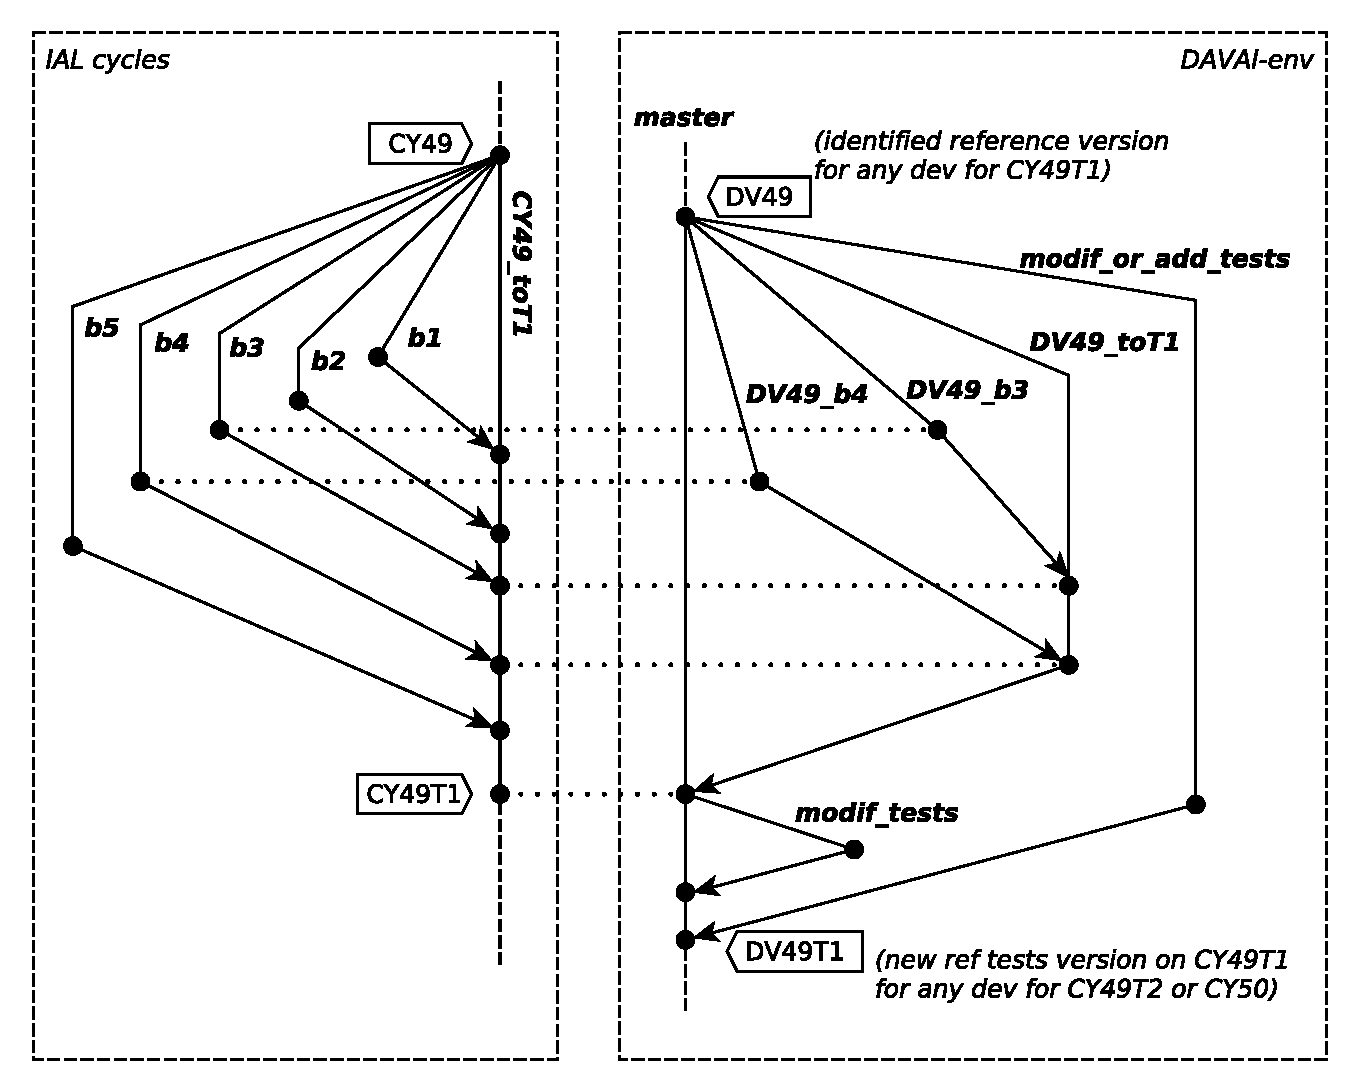
\includegraphics[scale=0.65]{../figures/tests_versioning.pdf}}
 \end{center}
 \caption{\label{fig:tests_versioning} Semi-parallel versioning of tests following cycles.}
\end{figure}



\subsection{When and in which branch to add/modify tests ?}

The tests modifications which are not intrinsically linked with a contribution (adding tests or modifying a test to modify its behaviour) can be done at any moment, in a development branch of the tests repository. However, in order not to disturb the users and integrators, they should be merged into the next official version of tests (i.e. the version used for contributions and integrations to IAL) only between a declaration of a IAL release and a call for contribution.

\newpage
\begin{appendix}

\section{Template: Integration Request by e-mail\label{appx:template}}

\vspace{1cm}

\textbf{BRANCH:} mary\_CY49\_superdev\\
\textbf{BASE in MF's S.C.R.:} CY49 (or commit if no tag)\\
\textbf{TARGET in MF's S.C.R.:} CY49T1\\
\textbf{AUTHOR(s):} A.Mary, G.Faure\\

\noindent\textbf{DOCUMENTATION:}\\
Scientific and technical doc, incl. namelist changes...\\

\noindent\textbf{NUMERICAL IMPACT:}\\
Kind of configurations, magnitude of impact, memory, CPU, or what bug it fixes, ...\\
Please mention "Bit-Reproducible" if so.\\

\noindent\textbf{VALIDATION EXPERIMENT:}\\
DAVAÏ experiment ID and link to Ciboulaï page if possible\\
Explanation in case of KO tests.\\

\noindent\textbf{SUGGESTED TECHNICAL REVIEWER:}\\
One or two suggested thematic expert(s) to review the technical implementation of the proposed contribution.\\

\noindent\textbf{MODIFIED SOURCE FILES:}\\
...\\

\noindent\textbf{DELETED SOURCE FILES:}\\
...\\

\noindent\textbf{RENAMED SOURCE FILES:}\\
...\\

\noindent\textbf{ADDED SOURCE FILES:}\\
...\\

\end{appendix}


\end{document}
